\documentclass{standalone}
\usepackage{tikz}
\usetikzlibrary{patterns,plotmarks}
\begin{document}
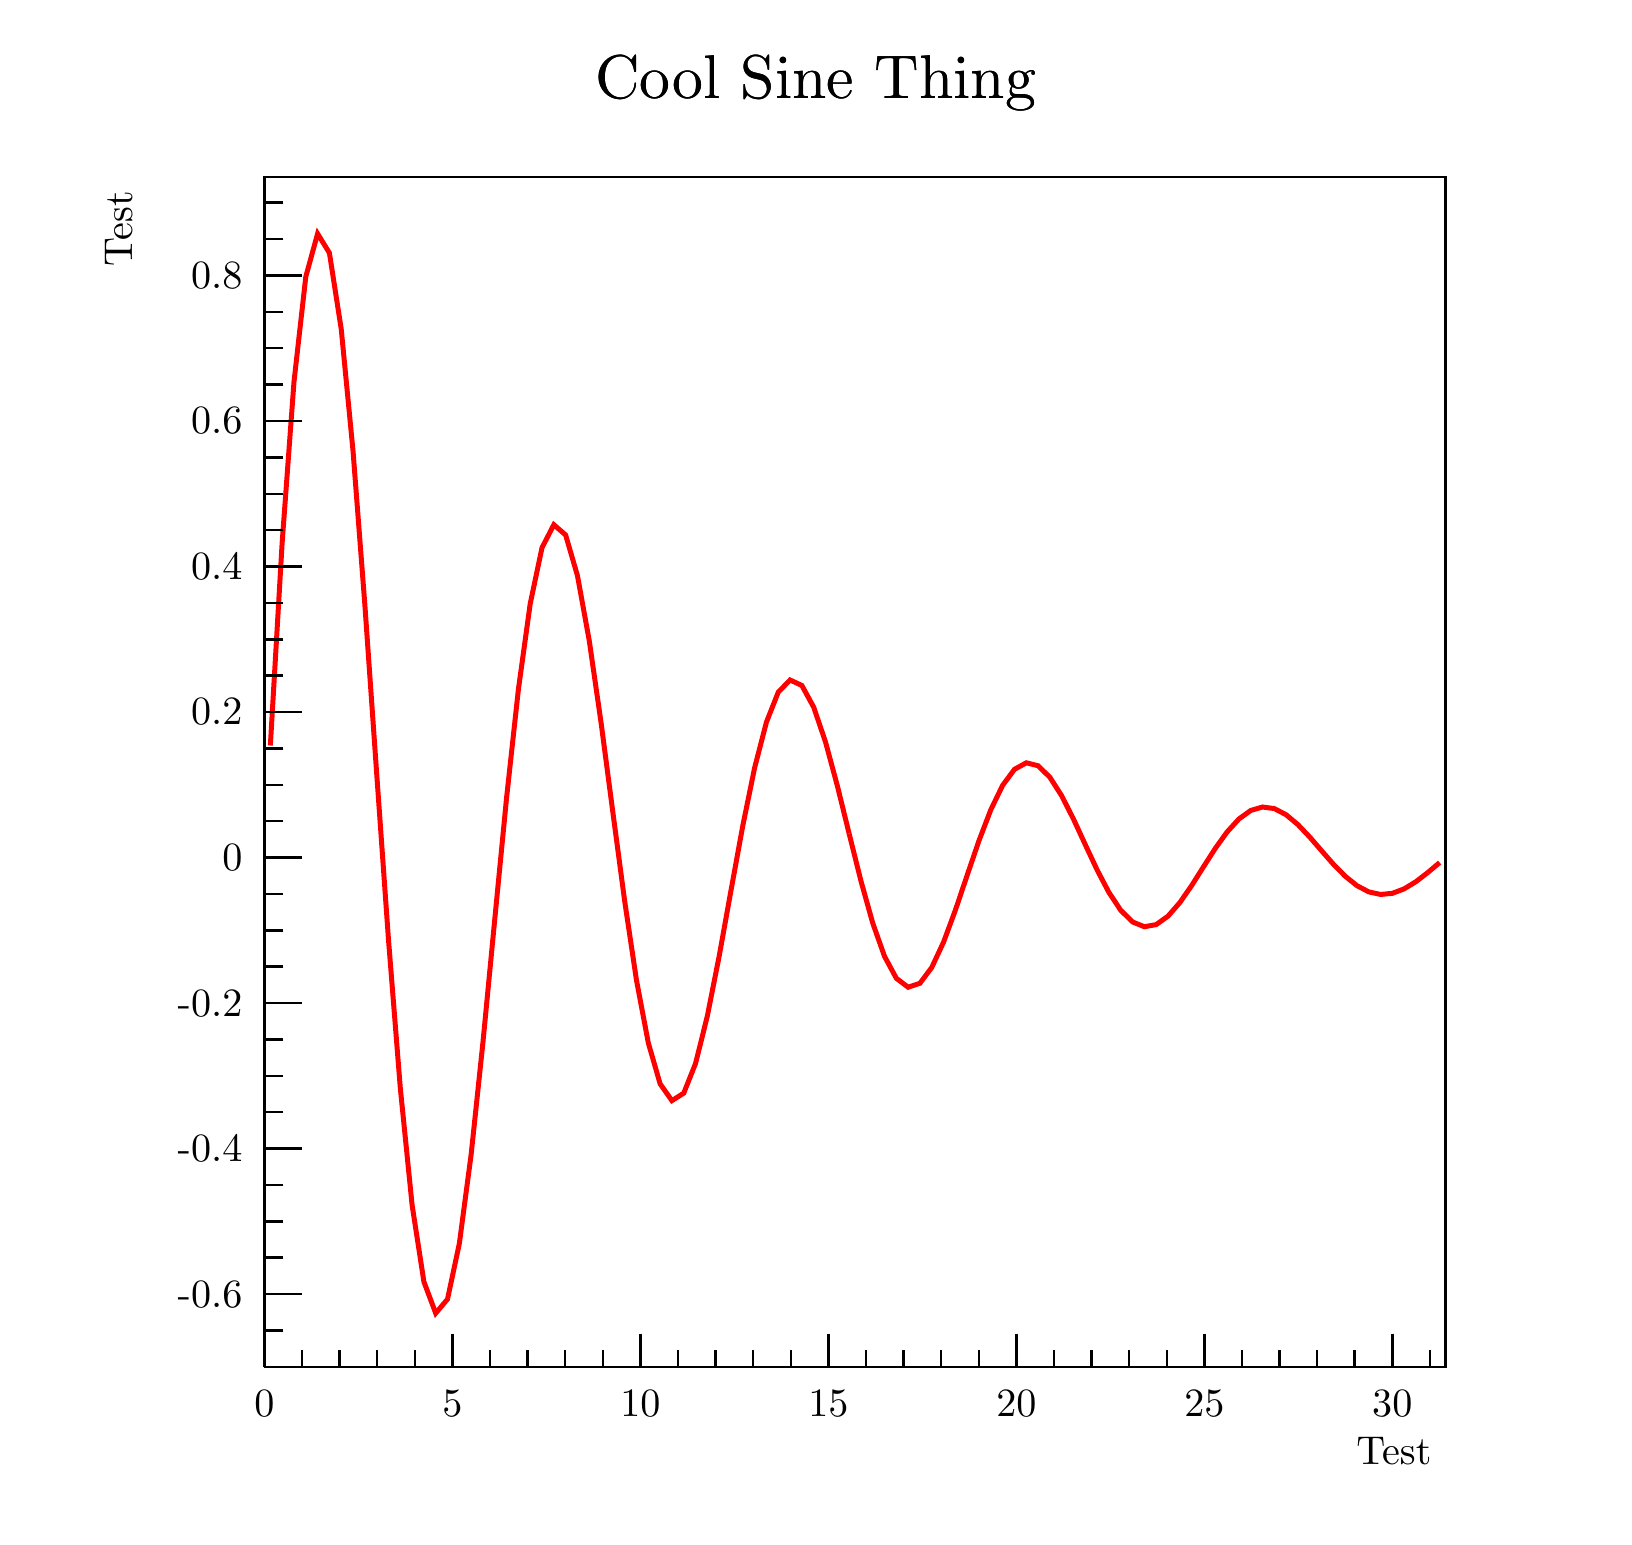
\begin{tikzpicture}
\def\CheckTikzLibraryLoaded#1{ \ifcsname tikz@library@#1@loaded\endcsname \else \PackageWarning{tikz}{usetikzlibrary{#1} is missing in the preamble.} \fi }
\CheckTikzLibraryLoaded{patterns}
\CheckTikzLibraryLoaded{plotmarks}
\pgfdeclareplotmark{cross} {
\pgfpathmoveto{\pgfpoint{-0.3\pgfplotmarksize}{\pgfplotmarksize}}
\pgfpathlineto{\pgfpoint{+0.3\pgfplotmarksize}{\pgfplotmarksize}}
\pgfpathlineto{\pgfpoint{+0.3\pgfplotmarksize}{0.3\pgfplotmarksize}}
\pgfpathlineto{\pgfpoint{+1\pgfplotmarksize}{0.3\pgfplotmarksize}}
\pgfpathlineto{\pgfpoint{+1\pgfplotmarksize}{-0.3\pgfplotmarksize}}
\pgfpathlineto{\pgfpoint{+0.3\pgfplotmarksize}{-0.3\pgfplotmarksize}}
\pgfpathlineto{\pgfpoint{+0.3\pgfplotmarksize}{-1.\pgfplotmarksize}}
\pgfpathlineto{\pgfpoint{-0.3\pgfplotmarksize}{-1.\pgfplotmarksize}}
\pgfpathlineto{\pgfpoint{-0.3\pgfplotmarksize}{-0.3\pgfplotmarksize}}
\pgfpathlineto{\pgfpoint{-1.\pgfplotmarksize}{-0.3\pgfplotmarksize}}
\pgfpathlineto{\pgfpoint{-1.\pgfplotmarksize}{0.3\pgfplotmarksize}}
\pgfpathlineto{\pgfpoint{-0.3\pgfplotmarksize}{0.3\pgfplotmarksize}}
\pgfpathclose
\pgfusepathqstroke
}
\pgfdeclareplotmark{cross*} {
\pgfpathmoveto{\pgfpoint{-0.3\pgfplotmarksize}{\pgfplotmarksize}}
\pgfpathlineto{\pgfpoint{+0.3\pgfplotmarksize}{\pgfplotmarksize}}
\pgfpathlineto{\pgfpoint{+0.3\pgfplotmarksize}{0.3\pgfplotmarksize}}
\pgfpathlineto{\pgfpoint{+1\pgfplotmarksize}{0.3\pgfplotmarksize}}
\pgfpathlineto{\pgfpoint{+1\pgfplotmarksize}{-0.3\pgfplotmarksize}}
\pgfpathlineto{\pgfpoint{+0.3\pgfplotmarksize}{-0.3\pgfplotmarksize}}
\pgfpathlineto{\pgfpoint{+0.3\pgfplotmarksize}{-1.\pgfplotmarksize}}
\pgfpathlineto{\pgfpoint{-0.3\pgfplotmarksize}{-1.\pgfplotmarksize}}
\pgfpathlineto{\pgfpoint{-0.3\pgfplotmarksize}{-0.3\pgfplotmarksize}}
\pgfpathlineto{\pgfpoint{-1.\pgfplotmarksize}{-0.3\pgfplotmarksize}}
\pgfpathlineto{\pgfpoint{-1.\pgfplotmarksize}{0.3\pgfplotmarksize}}
\pgfpathlineto{\pgfpoint{-0.3\pgfplotmarksize}{0.3\pgfplotmarksize}}
\pgfpathclose
\pgfusepathqfillstroke
}
\pgfdeclareplotmark{newstar} {
\pgfpathmoveto{\pgfqpoint{0pt}{\pgfplotmarksize}}
\pgfpathlineto{\pgfqpointpolar{44}{0.5\pgfplotmarksize}}
\pgfpathlineto{\pgfqpointpolar{18}{\pgfplotmarksize}}
\pgfpathlineto{\pgfqpointpolar{-20}{0.5\pgfplotmarksize}}
\pgfpathlineto{\pgfqpointpolar{-54}{\pgfplotmarksize}}
\pgfpathlineto{\pgfqpointpolar{-90}{0.5\pgfplotmarksize}}
\pgfpathlineto{\pgfqpointpolar{234}{\pgfplotmarksize}}
\pgfpathlineto{\pgfqpointpolar{198}{0.5\pgfplotmarksize}}
\pgfpathlineto{\pgfqpointpolar{162}{\pgfplotmarksize}}
\pgfpathlineto{\pgfqpointpolar{134}{0.5\pgfplotmarksize}}
\pgfpathclose
\pgfusepathqstroke
}
\pgfdeclareplotmark{newstar*} {
\pgfpathmoveto{\pgfqpoint{0pt}{\pgfplotmarksize}}
\pgfpathlineto{\pgfqpointpolar{44}{0.5\pgfplotmarksize}}
\pgfpathlineto{\pgfqpointpolar{18}{\pgfplotmarksize}}
\pgfpathlineto{\pgfqpointpolar{-20}{0.5\pgfplotmarksize}}
\pgfpathlineto{\pgfqpointpolar{-54}{\pgfplotmarksize}}
\pgfpathlineto{\pgfqpointpolar{-90}{0.5\pgfplotmarksize}}
\pgfpathlineto{\pgfqpointpolar{234}{\pgfplotmarksize}}
\pgfpathlineto{\pgfqpointpolar{198}{0.5\pgfplotmarksize}}
\pgfpathlineto{\pgfqpointpolar{162}{\pgfplotmarksize}}
\pgfpathlineto{\pgfqpointpolar{134}{0.5\pgfplotmarksize}}
\pgfpathclose
\pgfusepathqfillstroke
}
\definecolor{c}{rgb}{1,1,1};
\draw [color=c, fill=c] (0,0) rectangle (20,18.8945);
\draw [color=c, fill=c] (3,1.88945) rectangle (18,17.005);
\definecolor{c}{rgb}{0,0,0};
\draw [c,line width=0.9] (3,1.88945) -- (3,17.005) -- (18,17.005) -- (18,1.88945) -- (3,1.88945);
\definecolor{c}{rgb}{1,0,0};
\draw [c,line width=1.8] (3.075,9.78501) -- (3.225,12.3639) -- (3.375,14.4023) -- (3.525,15.7378) -- (3.675,16.2852) -- (3.825,16.0402) -- (3.975,15.0744) -- (4.125,13.5242) -- (4.275,11.5739) -- (4.425,9.43455) -- (4.575,7.32275) -- (4.725,5.43913)
 -- (4.875,3.95028) -- (5.025,2.97483) -- (5.175,2.57496) -- (5.325,2.75394) -- (5.475,3.45937) -- (5.625,4.5916) -- (5.775,6.01615) -- (5.925,7.57872) -- (6.075,9.12119) -- (6.225,10.497) -- (6.375,11.5844) -- (6.525,12.2969) -- (6.675,12.589) --
 (6.825,12.4583) -- (6.975,11.943) -- (7.125,11.116) -- (7.275,10.0755) -- (7.425,8.93423) -- (7.575,7.8076) -- (7.725,6.80271) -- (7.875,6.00843) -- (8.025,5.48804) -- (8.175,5.27471) -- (8.325,5.3702) -- (8.475,5.74654) -- (8.625,6.35057) --
 (8.775,7.11055) -- (8.925,7.94416) -- (9.075,8.76705) -- (9.225,9.50102) -- (9.375,10.0812) -- (9.525,10.4613) -- (9.675,10.6171) -- (9.825,10.5473) -- (9.975,10.2725) -- (10.125,9.83127) -- (10.275,9.27618) -- (10.425,8.66731);
\draw [c,line width=1.8] (10.425,8.66731) -- (10.575,8.06627) -- (10.725,7.53017) -- (10.875,7.10643) -- (11.025,6.82881) -- (11.175,6.715) -- (11.325,6.76594) -- (11.475,6.96671) -- (11.625,7.28895) -- (11.775,7.69439) -- (11.925,8.13912) --
 (12.075,8.57812) -- (12.225,8.96968) -- (12.375,9.27918) -- (12.525,9.48196) -- (12.675,9.56509) -- (12.825,9.52788) -- (12.975,9.38124) -- (13.125,9.14587) -- (13.275,8.84973) -- (13.425,8.52491) -- (13.575,8.20426) -- (13.725,7.91826) --
 (13.875,7.6922) -- (14.025,7.54409) -- (14.175,7.48338) -- (14.325,7.51055) -- (14.475,7.61766) -- (14.625,7.78957) -- (14.775,8.00587) -- (14.925,8.24312) -- (15.075,8.47733) -- (15.225,8.68622) -- (15.375,8.85134) -- (15.525,8.95952) --
 (15.675,9.00386) -- (15.825,8.98401) -- (15.975,8.90578) -- (16.125,8.78022) -- (16.275,8.62223) -- (16.425,8.44894) -- (16.575,8.27788) -- (16.725,8.1253) -- (16.875,8.0047) -- (17.025,7.92569) -- (17.175,7.8933) -- (17.325,7.90779) --
 (17.475,7.96493) -- (17.625,8.05665) -- (17.775,8.17204);
\draw [c,line width=1.8] (17.775,8.17204) -- (17.925,8.29861);
\definecolor{c}{rgb}{0,0,0};
\draw [c,line width=0.9] (3,1.88945) -- (18,1.88945);
\draw [c,line width=0.9] (3,2.31457) -- (3,1.88945);
\draw [c,line width=0.9] (3.47746,2.10201) -- (3.47746,1.88945);
\draw [c,line width=0.9] (3.95493,2.10201) -- (3.95493,1.88945);
\draw [c,line width=0.9] (4.43239,2.10201) -- (4.43239,1.88945);
\draw [c,line width=0.9] (4.90986,2.10201) -- (4.90986,1.88945);
\draw [c,line width=0.9] (5.38732,2.31457) -- (5.38732,1.88945);
\draw [c,line width=0.9] (5.86479,2.10201) -- (5.86479,1.88945);
\draw [c,line width=0.9] (6.34225,2.10201) -- (6.34225,1.88945);
\draw [c,line width=0.9] (6.81972,2.10201) -- (6.81972,1.88945);
\draw [c,line width=0.9] (7.29718,2.10201) -- (7.29718,1.88945);
\draw [c,line width=0.9] (7.77465,2.31457) -- (7.77465,1.88945);
\draw [c,line width=0.9] (8.25211,2.10201) -- (8.25211,1.88945);
\draw [c,line width=0.9] (8.72958,2.10201) -- (8.72958,1.88945);
\draw [c,line width=0.9] (9.20704,2.10201) -- (9.20704,1.88945);
\draw [c,line width=0.9] (9.68451,2.10201) -- (9.68451,1.88945);
\draw [c,line width=0.9] (10.162,2.31457) -- (10.162,1.88945);
\draw [c,line width=0.9] (10.6394,2.10201) -- (10.6394,1.88945);
\draw [c,line width=0.9] (11.1169,2.10201) -- (11.1169,1.88945);
\draw [c,line width=0.9] (11.5944,2.10201) -- (11.5944,1.88945);
\draw [c,line width=0.9] (12.0718,2.10201) -- (12.0718,1.88945);
\draw [c,line width=0.9] (12.5493,2.31457) -- (12.5493,1.88945);
\draw [c,line width=0.9] (13.0268,2.10201) -- (13.0268,1.88945);
\draw [c,line width=0.9] (13.5042,2.10201) -- (13.5042,1.88945);
\draw [c,line width=0.9] (13.9817,2.10201) -- (13.9817,1.88945);
\draw [c,line width=0.9] (14.4592,2.10201) -- (14.4592,1.88945);
\draw [c,line width=0.9] (14.9366,2.31457) -- (14.9366,1.88945);
\draw [c,line width=0.9] (15.4141,2.10201) -- (15.4141,1.88945);
\draw [c,line width=0.9] (15.8916,2.10201) -- (15.8916,1.88945);
\draw [c,line width=0.9] (16.369,2.10201) -- (16.369,1.88945);
\draw [c,line width=0.9] (16.8465,2.10201) -- (16.8465,1.88945);
\draw [c,line width=0.9] (17.3239,2.31457) -- (17.3239,1.88945);
\draw [c,line width=0.9] (17.3239,2.31457) -- (17.3239,1.88945);
\draw [c,line width=0.9] (17.8014,2.10201) -- (17.8014,1.88945);
\draw [anchor=base] (3,1.26593) node[scale=1.45088, color=c, rotate=0]{0};
\draw [anchor=base] (5.38732,1.26593) node[scale=1.45088, color=c, rotate=0]{5};
\draw [anchor=base] (7.77465,1.26593) node[scale=1.45088, color=c, rotate=0]{10};
\draw [anchor=base] (10.162,1.26593) node[scale=1.45088, color=c, rotate=0]{15};
\draw [anchor=base] (12.5493,1.26593) node[scale=1.45088, color=c, rotate=0]{20};
\draw [anchor=base] (14.9366,1.26593) node[scale=1.45088, color=c, rotate=0]{25};
\draw [anchor=base] (17.3239,1.26593) node[scale=1.45088, color=c, rotate=0]{30};
\draw [anchor= east] (18,0.831357) node[scale=1.45088, color=c, rotate=0]{Test};
\draw [c,line width=0.9] (3,1.88945) -- (3,17.005);
\draw [c,line width=0.9] (3.48,2.81801) -- (3,2.81801);
\draw [c,line width=0.9] (3.24,3.28002) -- (3,3.28002);
\draw [c,line width=0.9] (3.24,3.74202) -- (3,3.74202);
\draw [c,line width=0.9] (3.24,4.20403) -- (3,4.20403);
\draw [c,line width=0.9] (3.48,4.66603) -- (3,4.66603);
\draw [c,line width=0.9] (3.24,5.12804) -- (3,5.12804);
\draw [c,line width=0.9] (3.24,5.59004) -- (3,5.59004);
\draw [c,line width=0.9] (3.24,6.05204) -- (3,6.05204);
\draw [c,line width=0.9] (3.48,6.51405) -- (3,6.51405);
\draw [c,line width=0.9] (3.24,6.97605) -- (3,6.97605);
\draw [c,line width=0.9] (3.24,7.43806) -- (3,7.43806);
\draw [c,line width=0.9] (3.24,7.90006) -- (3,7.90006);
\draw [c,line width=0.9] (3.48,8.36207) -- (3,8.36207);
\draw [c,line width=0.9] (3.24,8.82407) -- (3,8.82407);
\draw [c,line width=0.9] (3.24,9.28607) -- (3,9.28607);
\draw [c,line width=0.9] (3.24,9.74808) -- (3,9.74808);
\draw [c,line width=0.9] (3.48,10.2101) -- (3,10.2101);
\draw [c,line width=0.9] (3.24,10.6721) -- (3,10.6721);
\draw [c,line width=0.9] (3.24,11.1341) -- (3,11.1341);
\draw [c,line width=0.9] (3.24,11.5961) -- (3,11.5961);
\draw [c,line width=0.9] (3.48,12.0581) -- (3,12.0581);
\draw [c,line width=0.9] (3.24,12.5201) -- (3,12.5201);
\draw [c,line width=0.9] (3.24,12.9821) -- (3,12.9821);
\draw [c,line width=0.9] (3.24,13.4441) -- (3,13.4441);
\draw [c,line width=0.9] (3.48,13.9061) -- (3,13.9061);
\draw [c,line width=0.9] (3.24,14.3681) -- (3,14.3681);
\draw [c,line width=0.9] (3.24,14.8301) -- (3,14.8301);
\draw [c,line width=0.9] (3.24,15.2921) -- (3,15.2921);
\draw [c,line width=0.9] (3.48,15.7541) -- (3,15.7541);
\draw [c,line width=0.9] (3.48,2.81801) -- (3,2.81801);
\draw [c,line width=0.9] (3.24,2.35601) -- (3,2.35601);
\draw [c,line width=0.9] (3.24,1.89401) -- (3,1.89401);
\draw [c,line width=0.9] (3.48,15.7541) -- (3,15.7541);
\draw [c,line width=0.9] (3.24,16.2161) -- (3,16.2161);
\draw [c,line width=0.9] (3.24,16.6781) -- (3,16.6781);
\draw [anchor= east] (2.9,2.81801) node[scale=1.45088, color=c, rotate=0]{-0.6};
\draw [anchor= east] (2.9,4.66603) node[scale=1.45088, color=c, rotate=0]{-0.4};
\draw [anchor= east] (2.9,6.51405) node[scale=1.45088, color=c, rotate=0]{-0.2};
\draw [anchor= east] (2.9,8.36207) node[scale=1.45088, color=c, rotate=0]{0};
\draw [anchor= east] (2.9,10.2101) node[scale=1.45088, color=c, rotate=0]{0.2};
\draw [anchor= east] (2.9,12.0581) node[scale=1.45088, color=c, rotate=0]{0.4};
\draw [anchor= east] (2.9,13.9061) node[scale=1.45088, color=c, rotate=0]{0.6};
\draw [anchor= east] (2.9,15.7541) node[scale=1.45088, color=c, rotate=0]{0.8};
\draw [anchor= east] (1.14422,17.005) node[scale=1.45088, color=c, rotate=90]{Test};
\draw (10,18.197) node[scale=2.23213, color=c, rotate=0]{Cool Sine Thing};
\draw (10,18.197) node[scale=2.23213, color=c, rotate=0]{Cool Sine Thing};
\end{tikzpicture}
\end{document}
